% This template has been tested with LLNCS DOCUMENT CLASS -- version 2.20 (10-Mar-2018)

% !TeX spellcheck = en-US
% !TeX encoding = utf8
% !TeX program = pdflatex
% !TeX TXS-program:compile = txs:///pdflatex/[--shell-escape]
% !BIB program = bibtex
% -*- coding:utf-8 mod:LaTeX -*-

% German documents: pass ngerman as class option
% \documentclass[ngerman,runningheads,a4paper]{llncs}[2018/03/10]
% English documents: pass english as class option
\documentclass[ngerman,runningheads,a4paper]{llncs}[2018/03/10]

\usepackage{improved-lncs}

\newcommand{\iu}{{i\mkern1mu}}

\begin{document}

\title{Subsurface scattering: Kombination von Theorie und Implementierungstechniken am Beispiel des realistischen Renderns von Haut}
%If Title is too long, use \titlerunning
\titlerunning{Realitische Echtzeitdarstellung von Haut}

%Single insitute
\author{Dennis Grabowski, B.Sc.}
%If there are too many authors, use \authorrunning
\authorrunning{D. Grabowski}

\institute{Hochschule Hannover, Ricklinger Stadtweg 120, 30459 Hannover, Germany\\
\email{dennis.grabowski@stud.hs-hannover.de}\\
\url{https://f4.hs-hannover.de/}}

\maketitle

\begin{abstract}

Unter dem typischen Phong-Modell ist es schwer, verschiedenste Materialien wie Marmor, Wachs, Blätter oder Haut realistisch dar\-zu\-stellen.
Zugrunde liegt, dass das Phong-Modell nur ein empirisches Model ist und keineswegs ein physikalisch haargenaues Modell darstellt, wodurch verschiedenste physikalische Effekte schlichtweg nicht nachstellbar sind.
Diese Ausarbeitung wird ausleuchten, welche Schwierigkeiten sich ergeben, Haut realistisch darzustellen und welche Konzepte helfen, diesen Realismus wiedergeben zu können.
Haut als Medium bietet sich besonders an, um an diese Konzepte heranzugehen, da jedem Leser hoffentlich eine realistische Präsentation dieser bekannt ist.
Hierfür wird zunächst aufgezeigt, wie Licht mit Haut interagiert, um die physikalischen Grundlagen der sogenannten Volumenstreuung (engl. subsurface scattering) kennenzulernen.
Anschliessend werden bestehende Techniken angeschnitten, die dieses physikalische Phänomen auf verschiedenste Weisen implementieren.
Durchleuchtet wird die sogenannte \enquote{Texture-space Diffusion}, welche bereits fuer den Film \enquote{The Matrix} verwendet wurde und von NVIDIA's d'Eon und Luebke fuer ein Echtzeit-Rendering-System adaptiert wurde.
Diese Technik verwendet die bidirektionale Reflexionsverteilungsfunktion von Kelemen und Szirmay-Kalos, um eine realistische Oberflächenreflexion zu simulieren, sowie Diffusionsprofile und Translucent Shadow Maps, um die Auswirkungen des Subsurface Scattering auf dem Hautmaterial nachzuahmen.

\end{abstract}

\begin{keywords}
  Computergrafik, Physikalisch-basiertes Rendering, Bidirektionale Reflexionsverteilungsfunktions (BRDFs), Subsurface scattering (deutsch Unterirdische Streuung/Volumenstreuung), Diffusionsprofile, Translucent shadow maps
\end{keywords}

\section{Einleitung}
\label{sec:intro}

Mithilfe des typischen Blinn-Phong-Modell ist schwer, Materialien wie Marmor, Wachs, Blaetter oder Haut realistisch darzustellen. Dies basiert auf dem Fakt, dass dies ein empirisches Modell ist, welches keineswegs versucht, in der Lage zu sein, alle physikalische Phaenomene nachstellen zu koennen.
Um die zuvorgenannten Materialien realistisch darstellen zu koennen, sind komplexere, physikalisch-fundierte Konzepte wie beispielsweise das \enquote{Subsurface Scattering}, zu deutsch \enquote{Volumenstreuung}, erforderlich.
Dieses physikalische Phaenomene beschreibt, wie Licht mit einem Objekt interagiert, nachdem es von diesem gebrochen aber nicht reflektiert wird.

Das Ziel dieser Ausarbeitung ist es, das Prinzip der Volumenstreuung vorzustellen und dem Leser einen Ueberblick ueber moegliche Techniken zu verschaffen, um dieses Phaenomen durch vorhandene Konzepte der Computergrafik entweder physikalisch korrekt darzustellen oder zu approximieren.

Hierfür werden zunächst die physikalische Grundlagen aufgefrischt, die noetig sind um die Volumenstreuung zu verstehen, und erklaert warum der Aufbau des Objekts einen Unterschied fuer die Streuung darstellen kann.
Damit diese Erklaerung relativ simpel bleiben kann, konzentriert sich diese Ausarbeitung auf Objekte, dessen Oberfläche aus dem Material \enquote{Haut} besteht.
Haut eignet sich besonders in diesem Kontext, da jedem Leser eine realistische Repraesentation dieses Materials wohl vertraut ist.
Nach Bewaeltigung der physikalischen Grundlagen werden 4 der bekanntesten realistischsten Haut-Render-Techniken vorgestellt, wovon der Fokus dieser Ausarbeitung auf der sogenannten \enquote{Texture-Space Diffusion} liegt, die bereits zum Film \enquote{The Matrix} Einsatz gefunden hat, und von NVIDIA's \citeauthor{advanced-realtime-skin-rendering} angepasst wurde, um in einem Echtzeit-Renderer verwendet werden zu koennen.

Diese Technik kombiniert die Anwendung der \enquote{bidirektionalen Reflexionsverteilungsfunktion} von Kelemen und Szirmay-Kalos mit der Anwendung von sogenannten \enquote{Diffusionsprofilen} und \enquote{Translucent Shadow Maps}, um die realistische Darstellung von Haut zu ermoeglichen.

Nachfolgend werden Bilder verschiedenster Implementationen sowie aktuellere Ergebnisse von \enquote{Offline-Renderern} miteinander vergliechen, um die Wirkung dieser Konzepte besser einschätzen zu können.

\section{Physikalische Grundlagen der Volumenstreuung}

Um die Volumenstreuung vollstaendig verstehen zu koennen, bedarf es zunaechst einer Auffrischung bezueglich der physikalischen Eigenschaften des Lichts und der generellen Lichtbrechung.

Licht ist eine Welle, die sich innerhalb eines Mediums (oder auch innerhalb eines Vakuums) geradlinig in eine Richtung fortbewegt.
In dieser Ausarbeitung bezeichnet Licht immer das fuer das menschliche Auge sichtbare Licht mit einer Wellenlaenge von ungefaehr 380 bis 800 nm. Andere elektromagnetische Strahlungen werden somit ignoriert.

Trifft eine Lichtwelle auf ein anderes Medium, so widerfaehrt es die Effekte der \enquote{Streuung} - es teilt sich in verschiedene Richtungen auf. Dadurch aendert sich nicht die gesamte Intensitaet, jedoch teilt sich die Intensitaet auf mehrere Lichtstrahlen auf.
Dabei werden die Lichtstrahlen entweder von der Oberfläche reflektiert, von der Oberfläche gebrochen oder absorbiert.
Die genauen Effekte des Eintreffens auf die Oberflaeche eines neuen Mediums haengt von mehreren Faktoren ab: dem Einfallswinkel des Lichts auf die Oberflaeche des Objekts, die Beschaffenheit der Oberflaeche und dem sogenannten \enquote{Brechnungsindex}.

Da diese Ausarbeitung abzielt, die Volumenstreuung zu erklaeren, wird von einer naeheren Erklaerung der Auswirkungen von Einfallswinkeln sowie Oberflächenbeschaffungen abgesehen, da diese sich eher auf eine Reflexion auswirken.

Der Brechnungsindex beschreibt das Verhaeltnis der Wellenlaenge des Lichts im Vakuum zur Wellenlaenge im Material und somit auch das Verhaeltnis der Phasengeschwindigkeit des Lichts im Vakuum zu der in dem betrachteten Material.
Es ist somit eine optische Eigenschaft eines Materials.
Besonders interessant ist die mathematische Darstellung dieses Index als komplexe Zahl: $$ \underline{n} = n + \iu * K$$
Der reelle Teil $n$ der komplexen Zahl beschreibt hierbei den Einfluss des Materials auf die Phasengeschwindigkeit des Lichts, wie stark das Licht durch das Material bei der Brechung verlangsamt wird, waehrend der imaginaere Teil $\iu * K$ den Massenschwaechungskoeffizienten beschreibt, ergo wie stark die Intensitaet des Lichts beim Propagieren durch das Material gedaempft wird.
Zusaetzlich laesst sich mithilfe des Snelliussches Brechungsgesetzes und des Brechnungsindex der Ausfallswinkel des gebrochenen Lichtstrahls in Relation zu dem Einfallswinkel des einfallenden Lichtstrahls berechnen.
Dadurch kann vorhergesagt werden, welchen Weg ein gebrochener Lichtstrahl innerhalb eines neuen Mediums nehmen wird - eine hilfreiche Eigenschaft fuer das Rendern solcher gebrochenen Lichtstrahlen ist.

Was genau jedoch einem gebrochenen Lichtstrahl widerfaehrt, haengt von der Art des ihn brechenden Mediums ab.
Metalle absorbieren die gebrochenen Lichtstrahlen vollstaendig und wandeln diese in Hitze um.
Nicht-Metalle, sogenannte Dielektrika, wiederum verhalten sich wie regulaere Medien - innerhalb dieser interagieren gebrochenen Lichtstrahlen mit den Partikeln des Materials wie Lichtstrahlen, die auf die Oberflaeche eines Mediums treffen - auch diese koennen absorbiert, wieder reflektiert, schlichtweg aus dem Objekt wieder emittiert werden oder sogar streuen.
Hierbei koennen die Dielektrika-Medien nach der Menge an unterschiedliche Brechnungsindexen gruppiert werden, wodurch sich die Auswirkungen eines gebrochenen Lichtstrahls fuer eine Vielzeit von Materialien zusammenfassen lassen.
Transparente Medien, beispielsweise Glass oder Wasser, haben nur einen gleichbleibenden Brechnungsindex, erlauben keine nennenswerte Absorption und lassen das Licht ohne Brechung durch sie passieren.
Homogene Medien, beispielsweise Bier, Kaffee, Wein oder Milch, haben zwar auch nur einen gleichbleibenden Brechnungsindex, jedoch absorbieren sie eine signifikante Menge des Lichts. Dadurch aendert sich nicht die Richtung, allerdings die Intensitaet des Lichts wodurch sich der Farbunterschied dieser Medien erklaeren laesst.
Heterogene Medien, beispielsweise Holz, Stein, Plastik, wiederum haben basierend auf strukturellen Aenderungen mehrere, unterschiedliche Brechnungsindexe. Diese strukturellen Aenderungen basieren entweder auf der Unreinheit eines Materials - Luftblasen, mikroskopisch, kleine Fremdpartikel oder aehnliches - oder basieren auf der Unterteilung in verschiedene Schichten, die wiederum alle aus verschiedenen Materialen bestehen.
Aendern sich die Brechnungsindexe eines heterogenen Mediums stetig, so wird das Licht gebogen.
Aendern sich diese jedoch abrupt, so streuen die Lichtstrahlen an jedem neuen Brechnungsindex.
Hierbei aendert sich die Richtung sowie die Intensitaet der Lichtstrahlen, jedoch kann es auch zu einer Absorption der Lichtstrahlen kommen.

Problematisch wird jedoch die Betrachtung von gebrochenen Lichtstrahlen im Falle einer komplexeren Materialbeschaffenheit eines Objekts, beispielsweise Haut - dem Fokus dieser Ausarbeitung.
Verschiedene Hautschichten bestehen aus verschiedenen Materialien, wodurch sich verschiedene, abrupt-wechselende Unterschiede in den Brechnungsindexen ergeben.
Jede neue Hautschicht absorbiert, reflektiert, bricht und streuut das Licht also auf ihre eigene Art und Weise.

Diese Streuung unterhalb der Oberfläche eines Objekts nennt sich \enquote{Subsurface scattering} oder zu deutsch \enquote{Volumenstreuung}.

\section{Subsurface scattering}
\label{sec:subsurface}

\begin{figure}[!h]
  \centering
  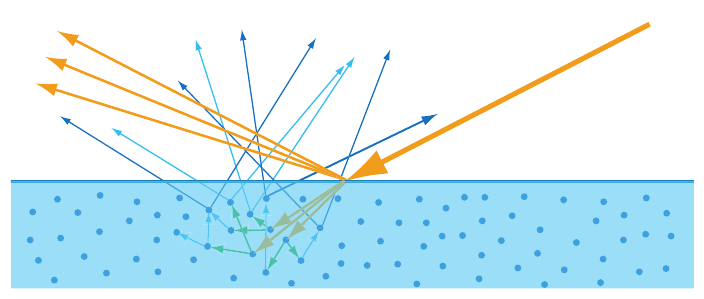
\includegraphics[scale=0.4,keepaspectratio]{./images/subsurface-scattering-illustration.jpg}
  \caption{Darstellung der Volumenstreuung in dielektrischen Materialien. Quelle: \cite{real-time-rendering}}
  \label{fig:subsurface-scattering}
\end{figure}

Die Volumenstreuung ist ein physikalisches Phaenomen, welches beschreibt, was mit gebrochenen Lichtstrahlen innerhalb eines Objekts passiert.
Hierbei treffen an der Oberflaeche des Objekts gebrochene Lichtstrahlen innerhalb des Objekts auf weitere, abrupte Aenderungen, wodurch die gebrochenen Lichtstrahlen ferner in eine Vielzahl von Lichtstrahlen mit potentiell unterschiedlichen Intensitaeten und potentiell allen moeglichen Richtungen aufgeteilt werden.
Die Verteilung dieser Streuung haengt von dem Typen des Materials ab und ist haeufig nicht uniform.

In Grafik \ref{fig:subsurface-scattering} wird dieser Effekt nochmal verdeutlicht. Der orangene Pfeil, der von oben rechts auf das neue Medieum faellt, ist ein einzeler Lichtstrahl, der bei der Interaktion an der Oberflaeche des Mediums streuut. Ein Teil, erkenntlich durch die 3 kleineren, orangenen Pfeile, die sich von dem Medium wieder entfernen, wird direkt von der Oberfläche reflektiert.
Die restlichen Lichtstrahlen werden mit der verbleibenden Intensitaet in verschiedenste Richtungen innerhalb des Mediums gebrochen und interagieren hierbei mit einzelnen Partikeln, die einen anderen Brechnungsindex haben, als das Medium, in welchem sie sich befinden.
Verfolgt man die gruenen Pfeile, so faellt auf, dass einige Lichtstrahlen vollstaendig von dem Medium absorbiert werden, wobei andere wieder von dem Objekt emittiert werden.
Hierbei muessen die wieder emittierten Lichtstrahlen nicht aus dem selben Punkt austreten, aus welchem sie ins Medium getreten sind. In der Grafik \ref{fig:subsurface-scattering-different-exit-point} wird nochmal verdeutlicht, wie stark der Austrittspunkt mancher der dargestellten Lichtstrahlen von dem Eintrittspunkt des ersten, einfallenden Lichtstrahls abweichen.

\begin{figure}[!h]
  \centering
  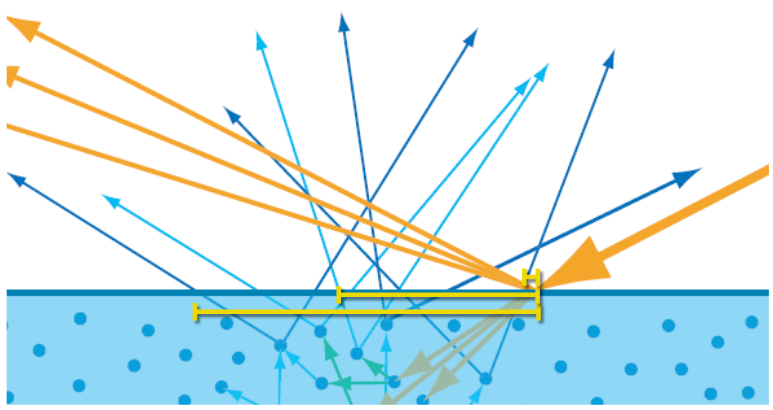
\includegraphics[scale=0.3,keepaspectratio]{./images/subsurface-scattering-distance-difference.jpg}
  \caption{Distanzunterschiede sind zwischen den Austrittspunkten und dem Eintrittspunkt zu erkennen. Quelle: \cite{real-time-rendering}}
  \label{fig:subsurface-scattering-different-exit-point}
\end{figure}

Aus den Grafiken \ref{fig:subsurface-scattering} und \ref{fig:subsurface-scattering-different-exit-point} ist ebenfalls erkenntlich, dass Lichtstrahlen unterschiedlich oft innerhalb eines Mediums streuen, bevor sie wieder von diesem Medium emittiert werden.
Man unterscheidet hierbei zwischen dem \enquote{Single-bounce scattering} und dem \enquote{Multiple-bounce scattering}; frei uebersetzt der einfachen Streuung und der mehrfachen Streuung.

\subsection{Konzeptionelle Adaptation der Volumenstreuung in der Computergrafik}

Appliziert man die eben gewonnenen Erkenntnisse auf die Computergrafik, so kann man die Distanzunterschiede der neu-emittierten Lichtstrahlen in Abhaengigkeit von Pixelgroessen darstellen, wie in Grafik \ref{fig:subsurface-scattering-pixel-considerations} dargestellt ist.

\begin{figure}[!h]
  \centering
  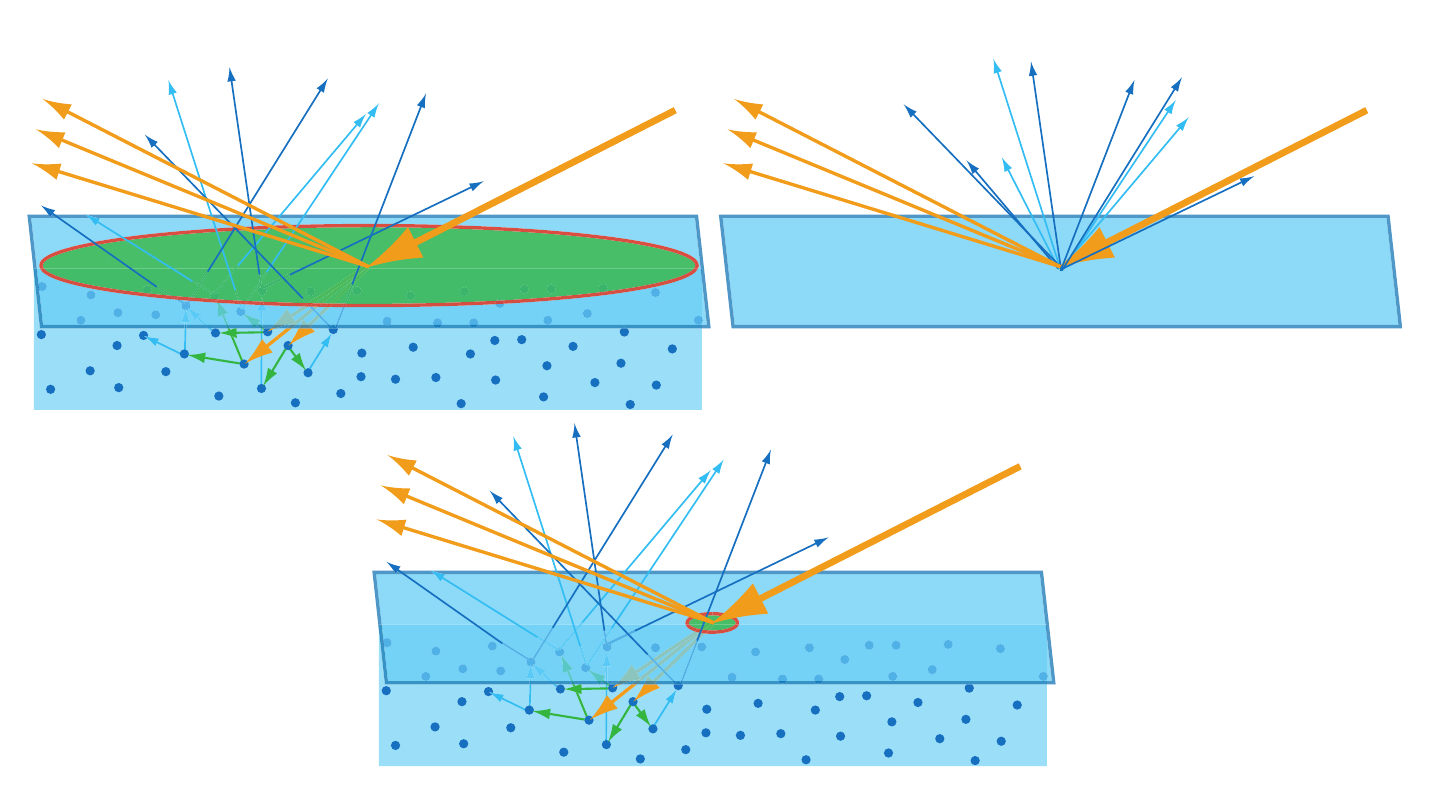
\includegraphics[scale=0.2,keepaspectratio]{./images/subsurface-scattering-pixel-considerations.jpg}
  \caption{Distanzunterschiede der neu-emittierten Lichtstrahlen in Abhaengigkeit verschiedener Pixelgroessen Quelle: \cite{real-time-rendering}}
  \label{fig:subsurface-scattering-pixel-considerations}
\end{figure}

Innerhalb dieser Grafik ist das bereits vorgestellte Beispiel zur Volumenstreuung um einen gruenen Kreis erweitert wurden, der die Groesse eines Pixels signalisieren soll.
Die linke Darstellung in der ersten Reihe zeigt somit ein Szenario, bei welchem die Distanz der Austrittspunkte der neu-emittierten Lichtstrahlen in Relation zu dem Eintrittspunkt des einfallenden Lichtstrahls kleiner ist als ein Pixel.
Dieses Szenario wird in der rechten Darstellung der ersten Reihe  vereinfacht dargestellt, in dem ein Renderer die Austrittspunkte in der Mitte des Pixels simuliert.
Die untere Abbildung zeigt den anderen Fall: Die Austrittspunkte sind ausserhalb des Pixels des einfallenden Lichtstrahls.

Diese Szenarien werden als lokale und globale Volumenstreuung kategorisiert.
Bei einer lokalen Volumenstreuung kann die Beleuchtung jedes Pixels individuell berechnet werden.
Dadurch ermoeglichen sich beispielsweise Performancegewinne durch Parallelitaet oder den Wechsel zu dieser Methode beim Rendern von weit entfernten Charakteren.
Implementiert werden lokale Volumenstreuungen normalerweise durch eine \enquote{Lambartische bidirektionale Reflektionsverteilungsfunktion}, die in der Lage ist, diffuse Reflektion mathematisch darzustellen. Diese Lambartischen BRDFs haben normalerweise folgende mathematische Definition: $f_diff(l, v) = c_diff / pi$
Eine oftmals praktischere Beschreibung kann durch die Applikation des Fresnelschen Effekts gewonnen werden: Specular reflectance increases at glancing angles, diffuse reflectance decreases: $f_diff(l, v) = (1 - R_F(Pho_i))  p_albedo/pi$
Typischerweise ignorieren diese BRDFs Einfluesse anderer Pixel, wodurch sie sich nicht bei einer Darstellung mit globalen Volumenstreuung eignen.
Bei einer globalen Volumenstreuung kann die Beleuchtung jedes Pixels potentiell die Beleuchtung jedes anderen Pixels des Bildes beeinflussen.
Diese Streuungen werden ueblicherweise durch \enquote{globale Beleuchtungsmodelle} wie beispielsweise \enquote{Raytracern} dargestellt.
Auch einer der Vorreiter der realistischsten Haut-Render-Techniken \citet{spectral-bssrdf-human-skin} bedarf sich dieser Methodik.
Fuer eine realistische Repraesentation ist ein Beleuchtungsmodell, welches globale Volumenstreuung beruecksichtigt, unumgaenglich und somit zwingend erforderlich.
Jedoch haben diese gewaltige Performanceimplikationen, wodurch Annaeherungen oder aehnliche \enquote{Tricks} angewendet werden muessen.

     math behind this only concerns radiance, i.e. magnitude of light along a single ray
       is a spectral quantity: amount varies as a function of wave length
       $L_i$ incoming to surface
       $L_o$ outgoing from surface
       $v$ denotes a unit-length vector pointing along the outgoing direction
       $l$ denotes a unit-length vector pointing opposite to the incoming direction
         it is more convenient to have all vectors point away from the surface
       $n$ denotes surface normal vector

\subsection{Struktur der Hautschichten}

Bevor die Vorstellung verschiedener Techniken zum realistischen Rendering des Materials Haut sinnvoll erscheint, sollte zunaechst untersucht werden, wie die menschliche Haut strukturiert ist und welche physikalischen Eigenschaften sie besitzt.

\begin{figure}[!h]
  \centering
  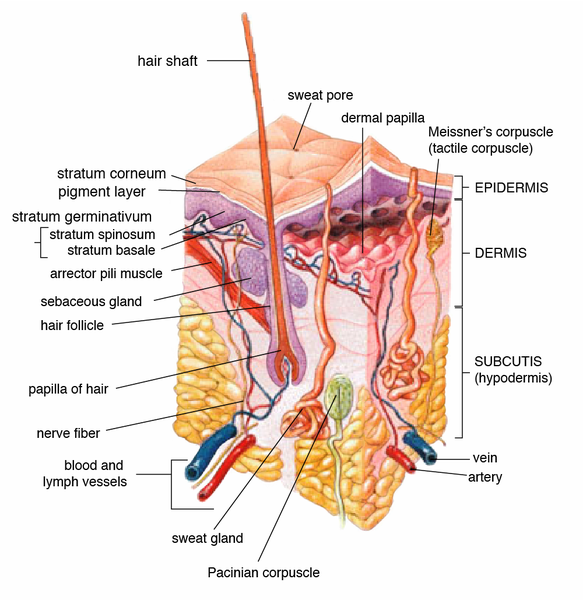
\includegraphics[scale=0.275,keepaspectratio]{./images/skin-layers-medical.png}
  \caption{Quelle: \url{https://en.wikipedia.org/wiki/File:Skin.png}}
  \label{fig:real-skin-layers}
\end{figure}

Die Grafik \ref{fig:real-skin-layers} zeigt eine medizinisch korrekte Darstellung der Zusammensetzung der unterschiedlichen Hautschichten. Die Haut ist somit ein heterogenes Medium.

Konzeptionell ist die Haut aufgeteilt in 3 Schichten: die Epidermis, die Dermis und die Hypodermis.
Direkt erkenntlich ist, dass sich die unterschiedlichen Schichten, keineswegs das Volumen der Haut uniform aufteilen.
Die Hypodermis und die Dermis machen einen hoeheren Anteil der Haut aus, waehrend die Epidermis hingegen die auesserste Schicht bildet, und somit als erstes mit einfallenden Lichtstrahlen interagiert.
In der Grafik leider nicht dargestellt ist das Sebum, eine oelige Substanz, die sich ueber Hautoberflaeche zieht und fuer ihren Glanz sorgt.
Ferner bestehen alle Schichten aus unterschiedlichen Materialien und sind von unterschiedlichen \enquote{Fremdpartikeln} durchzogen.
Haare oder Schweisporen strecken sich von der Hypodermis bis hin zur Epidermis.
Feine Venen und Arterien ziehen sich durch alle Schichten, um die Blutgefaesse der Haut mit ausreichend Blut versorgen zu koennen.
All diese Materialien verursachen, dass gebrochene Lichtstrahlen in die unterschiedlichsten Richtungen mit den unterschiedlichsten Intensitaeten gestreuut werden.
Eine exakte Repraesentation dieses Modells erweist sich daher als unhandlich fuer das realistische Rendering der Haut.

Laut \citeauthor{tuchin2015tissue} werden 6\% des einfallenden Lichts direkt an der Hautoberflaeche dank des Sebums reflekiert, waehrend die restlichen 94\% Lichtstrahlen innerhalb der Haut der Volumenstreuung unterliegen.
Fuer die reflektierten Lichtstrahlen ist hauptsaechlich das Sebum verantwortet.
Die Stratum Corneum ist hingegen hoechst streuuend, wodurch viele, multiple Streuungen stattfinden.
Ferner haben alle Bestandteile unterhalb der Dermis keinen nennenswerten Effekt auf die fuers menschliche Auge wahrgenommene Erscheinung \cite{tuchin2015tissue}.

Erforderlich ist somit ein Beleuchtungsmodell, dass den geringen Anteil der direkt reflektierten Lichtstrahlen und deren richtige Verteilung korrekterweise wiedergeben kann, sowie in der Lage ist eine globale Volumenstreuung zu simulieren.
Zu beruecksichtigen ist ferner, dass diese Eigenschaften ebenfalls approximiert werden koennten.

\section{Bekanntesten Techniken zum Rendern von realistischer Haut}
\label{sec:application}

\subsection{A Spectral BSSRDF for Shading Human Skin}
\label{sub:spectral-bssrdf}

\citet{spectral-bssrdf-human-skin}

 BSSRDF - bidirectional surface scattering distrubition function, by Jensen et al. 2001
         light distribution tends to be isotropic in a highly scattering media - i.e. once light is in the surface, it's randomly likely to end up coming out any direction rather being mostly aligned to the incoming light direction or any other similar possible dependency term
           this makes scattering sort of a blurring function
             comes from stam, 1995 - multiple scattering as a diffusion profile
           based on two parts:
             one method for exact computation of single-scattering contribution
             dipole method that approximates the multiple-scattering contribution by evaluating two virtual point light sources, one below and one above the surface

             BSSRDF is a generalization of a BRDF that is going to be applied as a global subsurface scattering method

             \begin{itemize}
              \item A global subsurface method scattering that evaluates a BSSRDF per pixel
              \item Uses Torrance-Sparrow (often also called Cook-Torrance) microfacet BRDF for surface reflection
              \item Uses a multipole diffusion model to calculate diffusion profiles that are used for subsurface scattering
            \end{itemize}

            Best visual representation but needs minutes to render a single image

            \begin{figure}[!h]
              \centering
              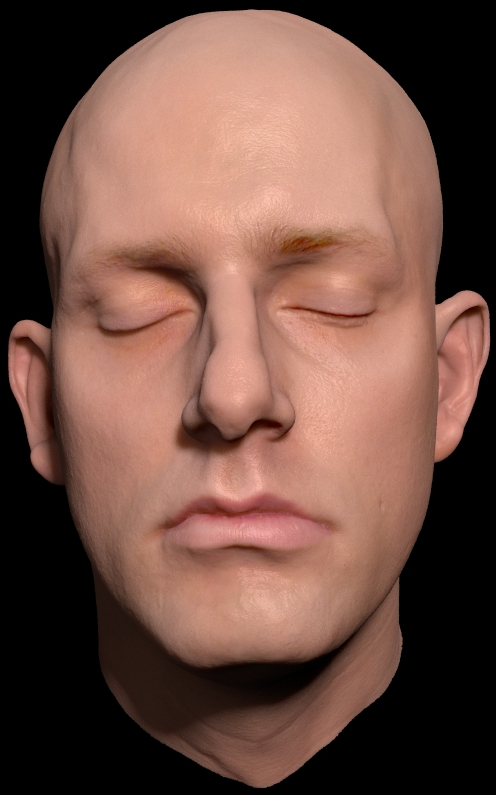
\includegraphics[scale=0.2,keepaspectratio]{./images/bssrdf-head.jpg}
              \caption{Source: \citet{spectral-bssrdf-human-skin}}
            \end{figure}

\subsection{Pre-Integrated Deferred Subsurface Scattering}
\label{sub:pre-integrated}

\citet{pre-integrated-subsurface}

PISS - Did not look that hard at this method, The Order: 1886 uses this.

\begin{figure}[!h]
  \centering
  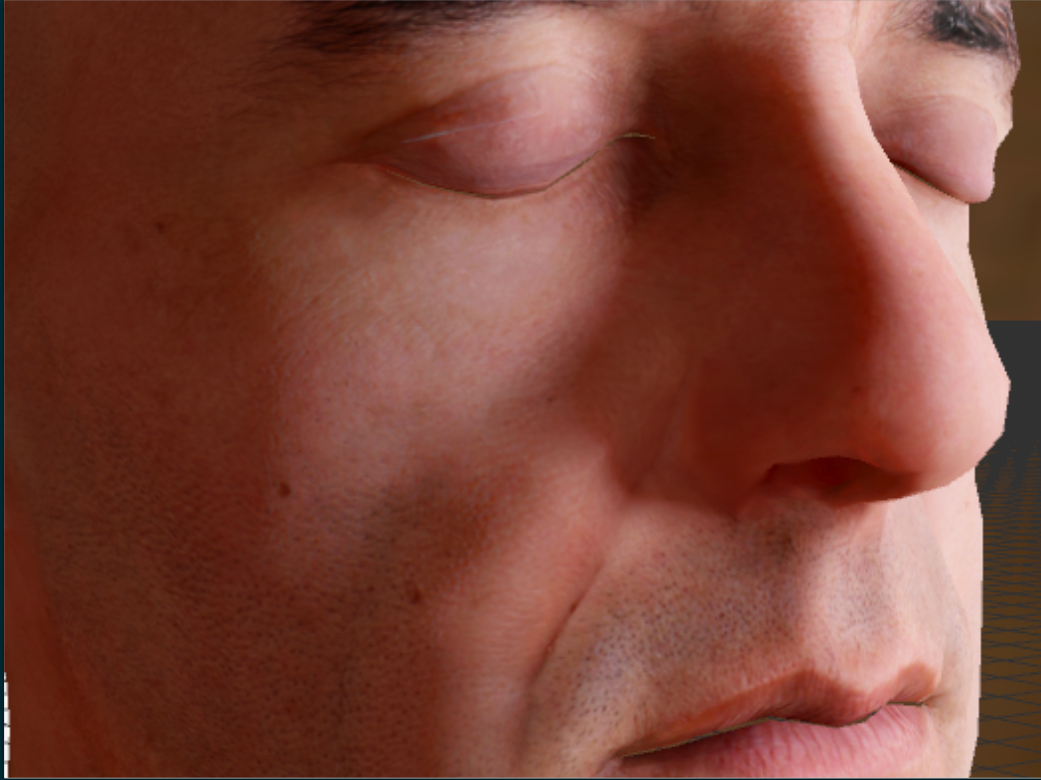
\includegraphics[scale=0.2,keepaspectratio]{./images/pre-integrated-ss.jpg}
  \caption{Source: \citet{pre-integrated-subsurface}}
\end{figure}

\subsection{Screen-space perceptual rendering of human skin}
\label{sub:screen-space}

\citet{screen-space-subsurface}

SSSS, also a global subsurface scattering method. Essentially does the same as the selected paper but in Screen-Space - Unity uses this, I think.

\begin{figure}[!h]
  \centering
  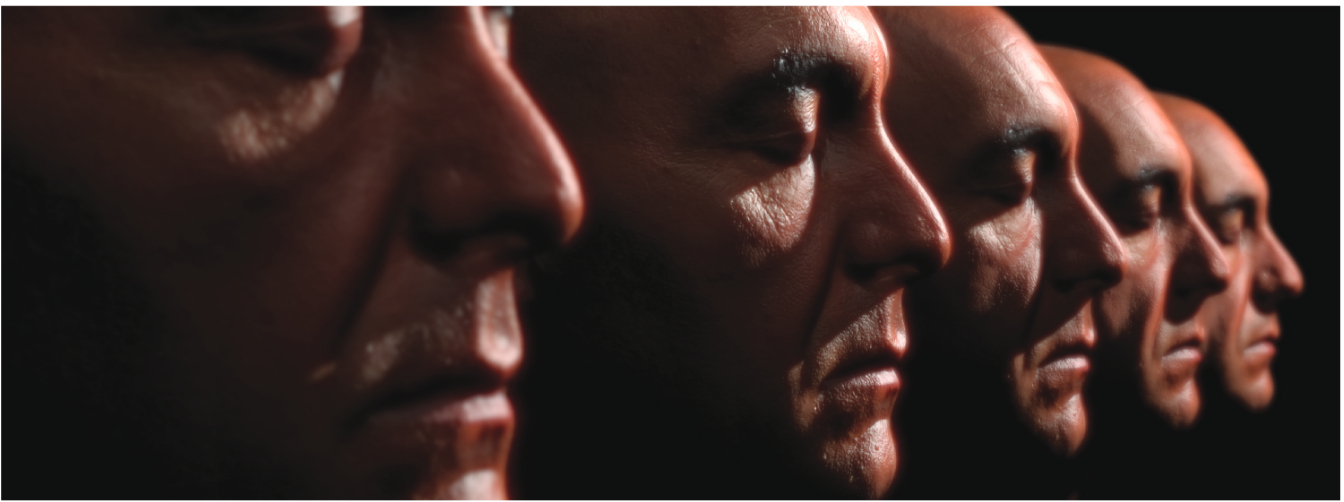
\includegraphics[scale=0.275,keepaspectratio]{./images/screen-space-sss.jpg}
  \caption{Source: \citet{screen-space-subsurface}}
\end{figure}

\begin{itemize}
  \item Ultimately uses the same technique as the paper we will be looking at, but in screen-space to maximize performance esp. when multiple actors are present.
  \item According to their psychological experiments, other users ranked their results on par with the paper we will be looking at.
\end{itemize}

\section{Texture-Space Diffusion}
\label{sec:texture-space}

 Texture-Space Diffusion
 based on an technique called Normal blurring
   an idea by Ma et al based on measured data that showed reflected lights from scattered objects specular reflecntance is based on geometric surface normals, diffuse reflectance behave as if it uses blurred surface normals
 a technique popularized by \citet{realistic-human-face-rendering-matrix} for the film Matrix formalizes the idea of multiple scattering as a blurring process of a texture
 Object mesh unwrapped onto a 2D texture
 surface irradiance aka diffuse lighting is rendered into a texture
   done by using texture coordinates as positions for rasterization.
   this texture is then blurred and used for diffuse shading when rendering
   shape/size of filter for blurring depends on material and wavelength
     for skin, a wider filter is used on R channel than on G or B channel causing the reddening near shadow edges
     most often, correct filter has narrow spike in the center, wide shallow base
     Reapplies blurred texture back onto the 3D model
     Subsurface scattering is therefore simulated by blurring
 this technique is very expensive, requiring large number of blurring passes - scaling back is possible for performance, but comes at a cost of realism

\citet{efficient-human-skin-rendering}
It's called "texture-space" because all of the scattering/diffusion simulation happens in 2D using the UV parameterization

\subsubsection{Skin model used}
\label{sub:skin-model}

\begin{figure}[!h]
  \centering
  \begin{minipage}{.5\textwidth}
    \centering
    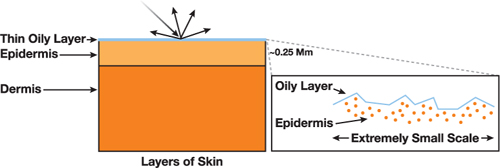
\includegraphics[scale=0.5,keepaspectratio]{./images/multilayer-skin-specular-reflection.jpg}
    \caption{Specular reflection in 3 layer skin model}
    \label{fig:test1}
  \end{minipage}%
  \begin{minipage}{.5\textwidth}
    \centering
    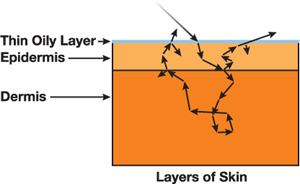
\includegraphics[scale=0.5,keepaspectratio]{./images/multilayer-skin-subsurface.jpg}
    \caption{Subsurface reflection in 3 layer skin model Source: \citet{advanced-realtime-skin-rendering}}
    \label{fig:test2}
  \end{minipage}
\end{figure}

\begin{figure}[!h]
  \centering
  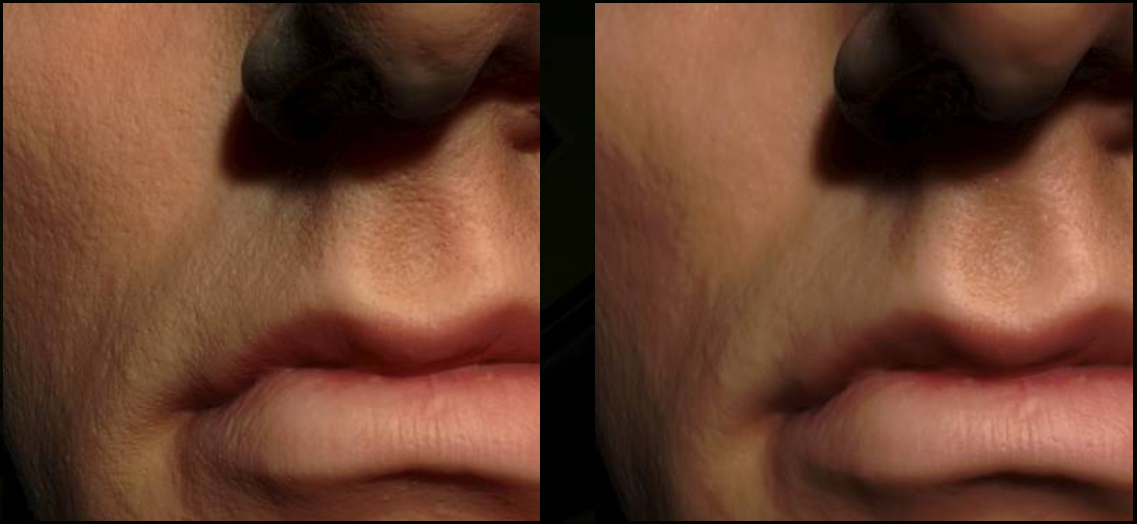
\includegraphics[scale=0.25,keepaspectratio]{./images/importance-of-layer-amount}
    \caption{Left: 3 layer skin model, Right: 1 layer skin model Source: \citet{efficient-human-skin-rendering}}
\end{figure}

Right side looks waxy

\subsection{Skin surface reflected light}
\label{sub:skin-surface-reflect}

Implemented by a BRDF created by Kelemen and Szirmay-Kalos.
Authors explain their choose for this BRDF to be due to performance reasons.
This BRDF seems to be easier on GPUs than the one Jensen uses in his BSSRDF (Cook-Terrance)

\begin{itemize}
  \item Kelemen \& Szirmay-Kalos BRDF used: $$f_{diff}(l, v) = albedo * \frac{(1 - R_{spec}(l))* (1 - R_{spec}(v))}{\pi * (1 - \overline{R_{spec}})}$$
  \begin{itemize}
    \item $R_{spec}$ = specular term of the BDRF (sometimes called directional albedo)
    \item $\overline{R_{spec}}$ = cosine-weighted integral over hemisphere
  \end{itemize}
\end{itemize}

scattering albedo p is ratio between energy of light that escapes a surface compared to energy of light entering into the material
value is between 0 (all light absorbed) and 1 (no light absorbed)
fresh snow or foam on liquid is good example of high scattering albedo - little absorption, immense scattering
good to know/consider is that albedo can have a different spectral distribution and thus color - think of plastic: reflecting specularly light is white, while reflecting diffusely will be colored by the pigment particles of the plastic (i.e. blue)
https://de.wikipedia.org/wiki/Albedo

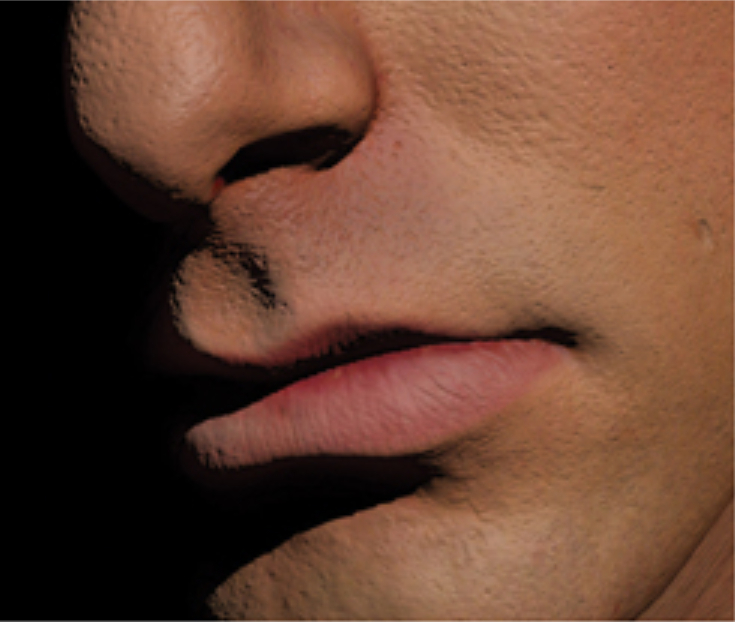
\includegraphics[scale=0.2,keepaspectratio]{./images/skin-rendering-without-sss.jpg}
\footnote{Formula taken from: \cite[p.~352]{real-time-rendering}, which in turn cites \cite{kelemen2001microfacet}}
\footnote{Image taken from: \citet{efficient-human-skin-rendering}}

\subsection{Skin subsurface reflected light}
\label{sub:skin-subsurface-reflect}

\subsubsection{Diffusion profiles}
\label{sub:diffusion-profiles}

\begin{itemize}
  \item Approximation for light scatter distribution underneath the surface of a highly scattering material
  \item Simple experiment: Illuminating a flat surface in a dark room with a thin, white laser beam.
  \item calculate diffusion profile as sum of gaussians
\end{itemize}

\begin{figure}[!h]
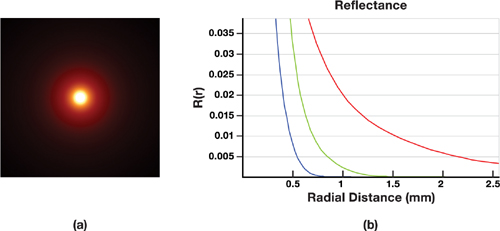
\includegraphics[scale=0.7,keepaspectratio]{./images/diffusion-profile-visualization}
\caption{TODO}
\end{figure}

\begin{itemize}
  \item We are seeing a glowing center which is due to the fact that some light rays are scattering through the surface and returning nearby
  \item This effectively tells us how much light emerges as a function of the angle and distance from laser center
  \item In uniform materials, scattering is the same in all materials, angle irrelevant
  \item Each color has it's own diffusion profile, as some might infer from the right-hand-side.
  \item Donner and Jenson are using 150 different diffusion profiles for their spectral BSSRDF
\end{itemize}

Diffusionprofile implementiert via einer Summe aus Gaussians

\begin{itemize}
  \item Definition of gaussian distribution: $G(v, r) = \frac{1}{2 * \pi * v} * e^{\frac{-r^{2}}{2*v}}$
  \item $R(r) = \sum\nolimits_{i=1}^k w_i * G(v_i, r)$
\end{itemize}

\begin{figure}[!h]
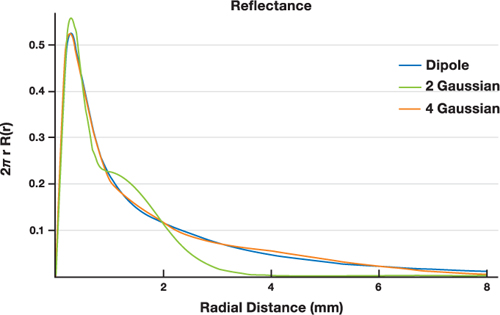
\includegraphics[scale=0.65,keepaspectratio]{./images/approximation-gaussians}
\caption{TODO}
\end{figure}

\begin{itemize}
  \item Authors saw a resembleance in the plotted curves to well-known Gaussian function $e^{-r^2}$
  \item Instead of measuring a diffusion profile for skin, the guys from NVIDIA, approximate the diffusion profile that Donner \& Jensen found in their research
  \item Sums of gaussians seemed to provide excellent Approximation
  \item Gaussians were used because they are simultaneously separable and radially symmetric
  \item $R(r)$ = a diffusion profile
  \item Constant factor in gaussian variance was chosen such that radial 2d blur does not darken or brighten the input image
  \item $r$ stands for radius
  \item find $k$ gaussians with different weights and variances
  \item Authors actually use a six gaussians summation to accurately match the three-layer model given in Donner/Jensen 2005
\end{itemize}

\subsubsection{Anwendung der Diffusionsprofile zur Simulation der Volumenstreuung}

\begin{figure}[!h]
  \centering
  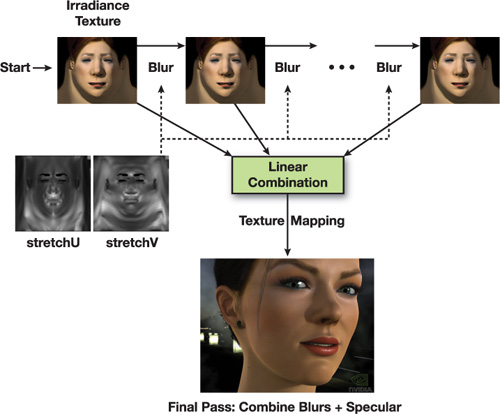
\includegraphics[scale=0.6,keepaspectratio]{./images/texture-space-algorithm.jpg}
  \caption{Source: \citet{efficient-human-skin-rendering}}
\end{figure}

\begin{itemize}
  \item Rasterize irradiance onto texture via vertex shader (U,V are texture coordinates)
  \item Compute lightning and fresnel terms in fragment shader (excluding specular)
  \item Ultimately more efficient as operations like convolutions can be performed more efficiently in image space
\end{itemize}

\begin{enumerate}
  \item Render shadow maps
  \item Render stretch correction map (optional: it may be precomputed).
  \item Render irradiance into off-screen texture.
  \item For each Gaussian kernel used in the diffusion profile approximation:
    \begin{itemize}
      \item Perform a separable blur pass in U (temporary buffer)
      \item Perform a separable blur pass in V (keep all of these for final pass).
    \end{itemize}
  \item Render mesh in 3D:
    \begin{itemize}
      \item Access each Gaussian convolution texture and combine linearly.
      \item Add specular for each light source.
    \end{itemize}
\end{enumerate}

\begin{figure}[!h]
  \centering
  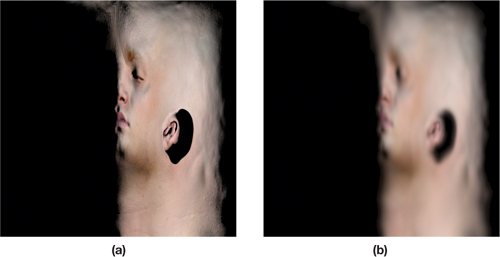
\includegraphics[scale=0.9,keepaspectratio]{./images/irradiance-texture-adrian.jpg}
  \caption{Source: \citet{efficient-human-skin-rendering}}
\end{figure}

\begin{figure}[!h]
  \centering
  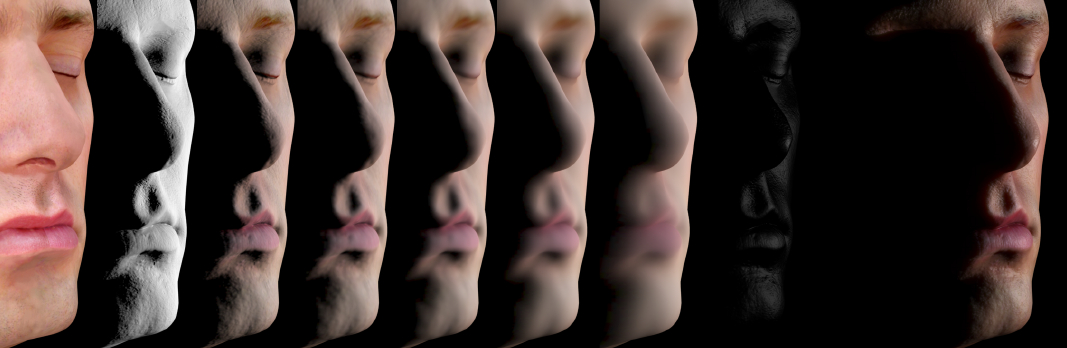
\includegraphics[scale=0.4,keepaspectratio]{./images/human-skin-final-rendering.jpg}
  \caption{Source: \citet{efficient-human-skin-rendering}}
\end{figure}

\begin{enumerate}
  \item First albedo,
  \item irradiance,
  \item Combine both to calculate subsurface irradiance,
  \item Do all gaussian blurs in texture space
  \item combine with specular
  \item produce final image!
  \item All convulutions are performed in 2d texture space but here mapped onto the face
\end{enumerate}

\subsubsection{Translucent shadow maps}
\label{sub:translucent-shadow-maps}

\begin{figure}
  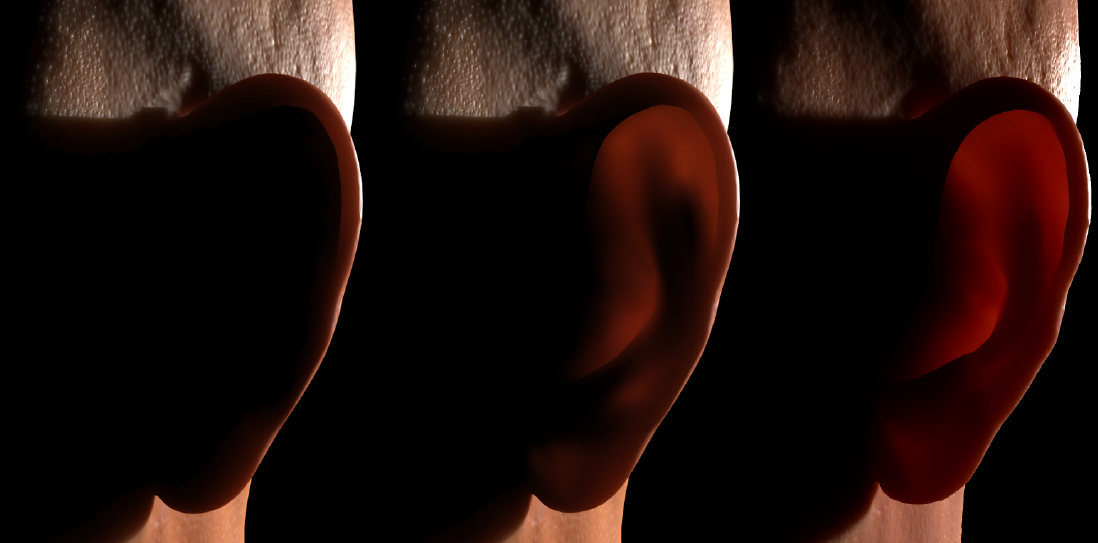
\includegraphics[scale=0.2,keepaspectratio]{./images/translucent-shadow-maps.jpg}
  \caption{
    Left: texture-space diffusion technique in thin skin regions,Center: rendering with translucent shadow maps for thin regions, Right: spectral BSSRDF model from Jensen et al. Source: \citet{efficient-human-skin-rendering}
  }
\end{figure}

\citet{translucent-shadow-maps}

\begin{itemize}
  \item Use translucent shadow maps
  \item On ears, nostrils and other thin skin regions the two surface locations are very close in 3D space, but not in texture space which does not correctly calculate the subsurface scattering
  \item \citeauthor{efficient-human-skin-rendering} modified the original maps to allow for a very efficient estimate of diffusion through thin regions by reusing convolved irradiance textures.
  \item Look into my paper for more, think the time is too narrow to go into this.
\end{itemize}

\section{Conclusion and Outlook}
\label{sec:outlook}

\begin{figure}[!h]
  \centering
  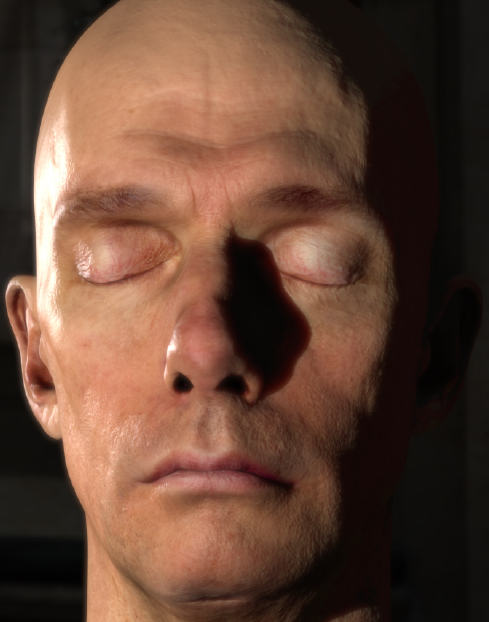
\includegraphics[scale=0.275,keepaspectratio]{./images/nvidia-result.jpg}
  \caption{Source: \citet{efficient-human-skin-rendering}}
\end{figure}

\begin{figure}[!h]
  \centering
  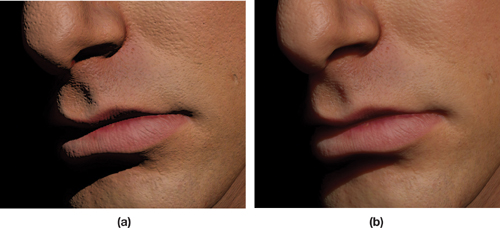
\includegraphics[scale=0.9,keepaspectratio]{./images/skin-rendering-with-without-sss.jpg}
  \caption{Source: \citet{efficient-human-skin-rendering}}
\end{figure}

\begin{figure}
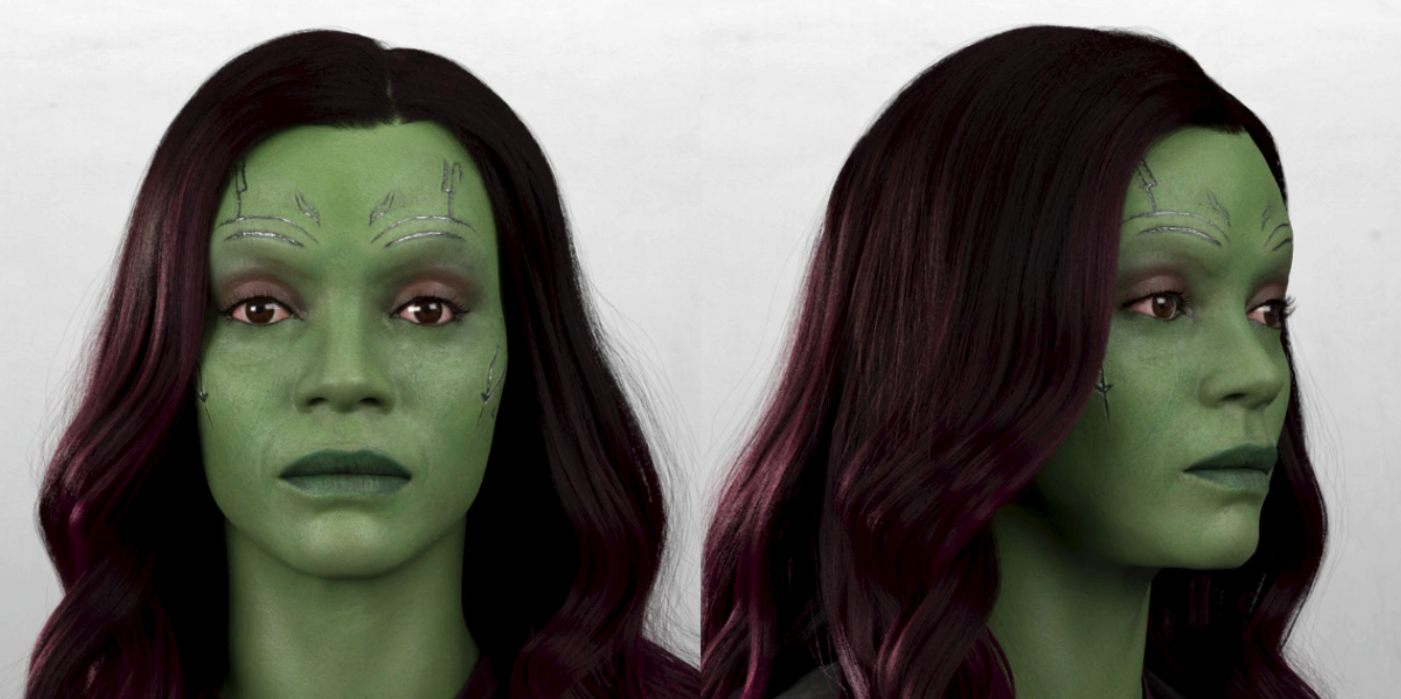
\includegraphics[scale=0.275,keepaspectratio]{./images/framestore-digital-gamora.jpg}
\caption{Volumetric path tracer - technique used by Framestore \protect\footnotemark}
\footnotetext{Quelle: \url{https://blog.selfshadow.com/publications/s2017-shading-course/walster/s2017_pbs_volumetric_notes.pdf}}
\end{figure}

\begin{itemize}
  \item Framestore is a high-end VFX studio, which did GotG2 and Alien: Covenant effects.
  \item Computationally highly expensive - not usable for anything interactive currently.
\end{itemize}

\begin{figure}
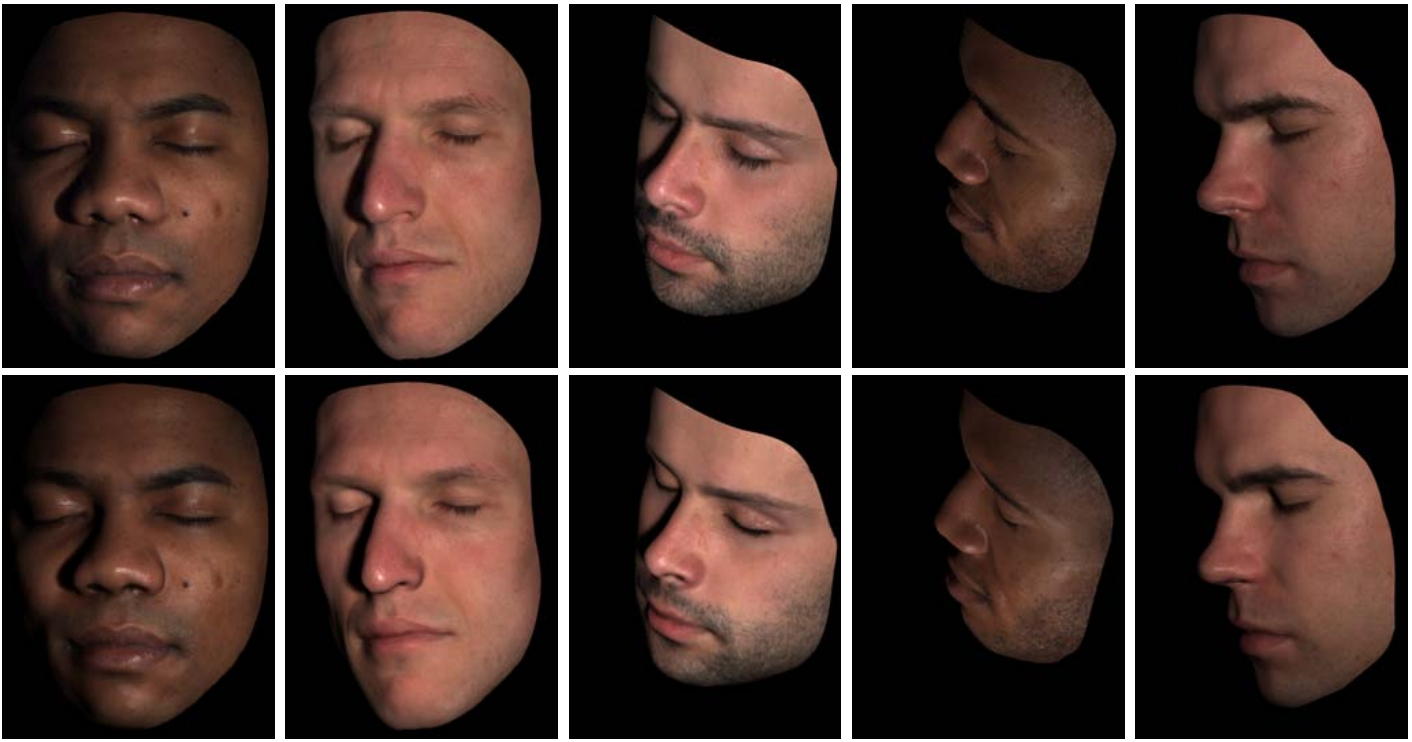
\includegraphics[scale=0.275,keepaspectratio]{./images/monte-carlo-ray-tracer.jpg}
\caption{A \enquote{Monte Carlo offline ray tracer} implemented in \citet{weyrich2006analysis}. Top row shows photograph, bottom shows rendered images}
\end{figure}

\renewcommand{\bibsection}{\section{Referenzen}} % requried for natbib to have "References" printed and as section, not chapter
% Use natbib compatbile splncsnat style.
% It does provide all features of splncs03, but is developed in a clean way.
% Source: http://phaseportrait.blogspot.de/2011/02/natbib-compatible-bibtex-style-bst-file.html
\bibliographystyle{splncsnat}
\begingroup
  \ifluatex
    %try to activate if bibliography looks ugly
    %\sloppy
  \else
    \microtypecontext{expansion=sloppy}
  \fi
  \small % ensure correct font size for the bibliography
  \bibliography{paper}
\endgroup

% Enforce empty line after bibliography
\ \\
%
All links were last followed on May 21, 2020.
\end{document}
